%sec1: comment trouve-t-on les surprises
%sec2: surprises and sale dynamics
%sec3: precision of the prior

%Sales of movies with positive surprise and sales of movies with negative surprise should diverge over time. To test this, we need to regress the log of sales on time and the interaction between time and surprise. If the coefficient of the interaction between time and surprise is significantly positive, then the sales of movies with positive surprise decrease slower than the sale of movies with negative surprise. If our results are consistent with those of Moretti, we should find that controlling for advertising, critic reviews and other variables does not affect significantly the results.

% The effect of a surprise should be lower for movies with a more precise prior. To test this, we augment the previous regression equation with the interaction of time and the precision of the prior and the interaction of time, precision of the prior and surprise of the movie (whose coefficient is predicted to be negative). The precision of the prior can be a dummy for sequels (sequels are assumed to have a more precise prior) or can be measured by the variance of the first week surprise for movies of the same genre.

Moretti's purpose is to provide evidence of social learning in consumption, that is to say that people tend to take into account their peers' experience to get a more precise idea of the value of a good. Economists, Moretti says, have had difficulties showing such social learning effects because of the absence of useful microdata on the matter. Moretti's innovation lies in his use of market-level data to identify social learning. He does so by defining what he calls ``surprises'' in movie sales: surprises, as their name suggests, consist in the difference between expected and actual sales. Moretti proposes that if we observe a surprise, we should also observe social learning effects: if a film is better or worse than expected, then by gathering experience through peers, people should reconsider their expectations and we might be able to see it in the data. In particular, Moretti makes five predictions on things we should be able to observe in presence of social learning: \begin{enumerate}
	\item in presence of social learning, sales of movies with positive and negative surprises should diverge: sales of better-than-expected movies should decrease at a lower rate than worse ones (see \ref{subsec2.2}); 
	\item we should observe less social learning effects from a movie on which quality we have a precise idea and more social learning effects from movies which have a more uncertain quality (see \ref{subsec2.3});
	\item we should observe more social learning effects when people have a greater social network (see \ref{subsec2.4});
	\item we should be able to observe that the effects of a surprise decline over time: once the information on the quality of a movie has been shared, what was a surprise should not play a major role in sales (see \ref{subsec2.5});
	\item we should not observe social learning effects when a surprise is due to elements other than quality of the film (let say weather).
\end{enumerate}
We have replicated Moretti's work and tried to confront his predictions with French data.
\pagebreak
\subsection{Identification of the surprises}\label{subsec2.1}

Surprises consist in the residuals of the regression of the log-number of sales in the first week on the log-number of screens available (opened by theaters). This definition of surprises holds because we suppose that theaters are profit-maximizing agents and make use of all the available information to predict the success of a movie. If this definition is correct, we should expect log-number of screens opened by theaters first week to be a good indicator of knowledge available on the movie quality before it is released. In the Table \ref{part2.1_tab1} we reproduce Moretti's regression of \textit{log\_sales\_first\_we} on \textit{log\_screens\_first\_week}. Each column is the result of the regression when we control with some variables (film genre, rating available, cost, distributor, weekday, month, week, year). The fact that adding control variables doesn't change the robustness of the regression proves Moretti's point which is that theaters take into account these factors when deciding their number of available screens. 

\begin{table}[!htbp] \centering 
	\caption{Regression of first-weekend sales on number of screens} 
	\label{part2.1_tab1} 
	\begin{tabular}{@{\extracolsep{5pt}}lccccccc} 
		\\[-1.8ex]\hline 
		\hline \\[-1.8ex] 
		& \multicolumn{7}{c}{\textit{Dependent variable:}} \\ 
		\cline{2-8} 
		\\[-1.8ex] & \multicolumn{7}{c}{log\_sales\_first\_we} \\ 
		\\[-1.8ex] & (1) & (2) & (3) & (4) & (5) & (6) & (7)\\ 
		\hline \\[-1.8ex] 
		log\_screens\_first\_week & 0.893$^{***}$ & 0.896$^{***}$ & 0.883$^{***}$ & 0.871$^{***}$ & 0.803$^{***}$ & 0.806$^{***}$ & 0.813$^{***}$ \\ 
		& (0.004) & (0.005) & (0.005) & (0.005) & (0.006) & (0.006) & (0.006) \\ 
		& & & & & & & \\ 
		\hline \\[-1.8ex] 
		R$^{2}$ & 0.907 & 0.909 & 0.910 & 0.912 & 0.932 & 0.936 & 0.938 \\ 
		Adjusted R$^{2}$ & 0.907 & 0.908 & 0.910 & 0.912 & 0.928 & 0.931 & 0.933 \\ 
		\hline 
		\hline \\[-1.8ex] 
		\textit{Note:}  & \multicolumn{7}{r}{$^{*}$p$<$0.1; $^{**}$p$<$0.05; $^{***}$p$<$0.01} \\ 
	\end{tabular} 
\end{table} 
%In fact, theaters perform more than what we could do using all the data available in the data set. Regressing first week-end sales on our control variables gives us a R\textsuperscript{2} of .7, which is smaller than .9 performed by theaters only.
%\todo{is this useful?}
%\todo{nope, you only need the significativity of the coefficient}
%\begin{table}[!htbp] \centering 
%	\caption{Regression of first-weekend sales on control variables} 
%	\label{part2.1_tab2} 
%	\begin{tabular}{@{\extracolsep{5pt}}lc} 
%		\\[-1.8ex]\hline 
%		\hline \\[-1.8ex] 
%		& \multicolumn{1}{c}{\textit{Dependent variable:}} \\ 
%		\cline{2-2} 
%		\\[-1.8ex] & log\_sales\_first\_we \\ 
%		\hline \\[-1.8ex] 
%		\hline \\[-1.8ex] 
%		Observations & 4,992 \\ 
%		R$^{2}$ & 0.699 \\ 
%		Adjusted R$^{2}$ & 0.674 \\ 
%		\hline 
%		\hline \\[-1.8ex] 
%		\textit{Note:}  & \multicolumn{1}{r}{$^{*}$p$<$0.1; $^{**}$p$<$0.05; $^{***}$p$<$0.01} \\ 
%	\end{tabular} 
%\end{table}

We have performed the same kind of regression on France data from 2004 to 2008 and find quite similar results (see table \ref{part2.1_tab3}).
\begin{table}[H] \centering 
	\caption{Regression of first-week entries on number of screens for France} 
	\label{part2.1_tab3} 
	\begin{tabular}{@{\extracolsep{5pt}}lccccccc} 
		\\[-1.8ex]\hline 
		\hline \\[-1.8ex] 
		& \multicolumn{7}{c}{\textit{Dependent variable:}} \\ 
		\cline{2-8} 
		\\[-1.8ex] & \multicolumn{7}{c}{log\_entree\_fr} \\ 
		\\[-1.8ex] & (1) & (2) & (3) & (4) & (5) & (6) & (7)\\ 
		\hline \\[-1.8ex] 
		log\_seance\_fr & 1.208$^{***}$ & 1.237$^{***}$ & 1.237$^{***}$ & 1.279$^{***}$ & 1.282$^{***}$ & 1.287$^{***}$ & 1.196$^{***}$ \\ 
		& (0.009) & (0.010) & (0.010) & (0.014) & (0.014) & (0.014) & (0.014) \\ 
		& & & & & & & \\ 
		\hline \\[-1.8ex] 
%		Observations & 2,046 & 2,046 & 2,046 & 2,046 & 2,046 & 2,046 & 2,046 \\ 
		R$^{2}$ & 0.893 & 0.899 & 0.900 & 0.917 & 0.924 & 0.925 & 0.943 \\ 
		Adjusted R$^{2}$ & 0.893 & 0.898 & 0.898 & 0.910 & 0.915 & 0.916 & 0.935 \\ 
		\hline 
		\hline \\[-1.8ex] 
		\textit{Note:}  & \multicolumn{7}{r}{$^{*}$p$<$0.1; $^{**}$p$<$0.05; $^{***}$p$<$0.01} \\ 
	\end{tabular} 
\end{table} 
We can see that the number of sales in first week is highly explained by the number of screens opened. This result holds even when adding controls: each column corresponds to a regression in which we added a control variable (genre, ratings, distributors, month and week, year, and some other variables).  


\subsection{Divergence of the sales}\label{subsec2.2}


The first prediction of Moretti is that if there are social learning effects in movie sales, we should observe diverging trajectories between movies with positive and negative surprises. The idea is simple: without social learning, sales of movies with positive and negative surprises should decrease at the same rate; in other words, surprises would not have any effect on sales. Indeed, people would not take surprises as a new information on the movie quality. In the figure \ref{part2.1_plot_moretti}, we have reproduced Moretti's graph and plotted the graph for French data. In Moretti's graph we clearly see the diverging trajectories of the sales. Our graph shows less clear diverging trajectories on the whole durations we computed, though it is clear that trajectories diverge in the first four weeks of projections.
\begin{figure}[H]\centering
	\caption{Comparing decline in sales between Moretti's and French data}
	\label{part2.1_plot_moretti}
	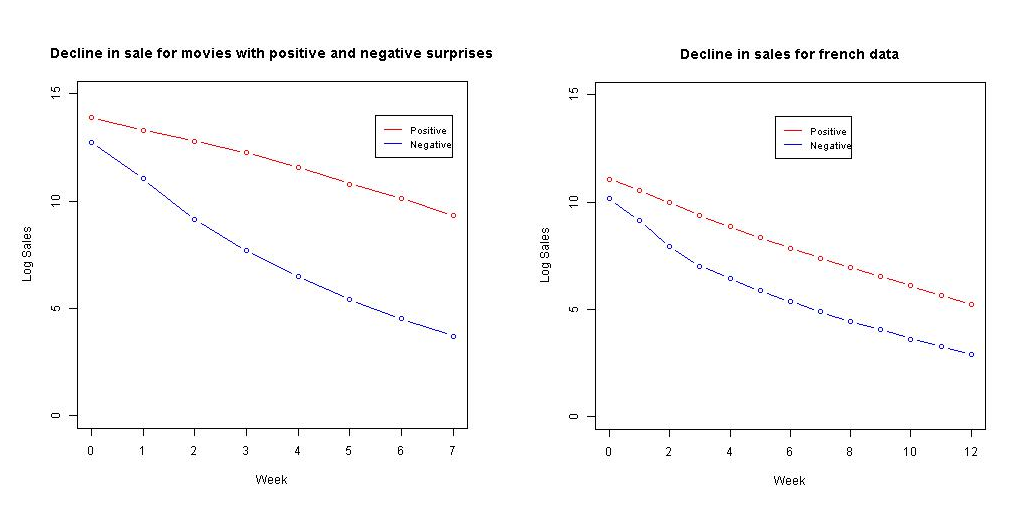
\includegraphics[scale=0.6]{comparison.png}
\end{figure}
\noindent To test for differences in trajectories, Moretti estimates models of the form: \begin{equation}\label{eq_divergence}
\ln(y_{jt})=\beta_0+\beta_1*t+\beta_2(t*S_j)+d_j+u_{jt}
\end{equation}
where $\ln(y_{jt})$ is the log of box-office sales in week $t$; $S_j$ is surprise; $d_j$ is a movie fixed effect. The variable of interest is $\beta_2$ because we want to identify an effect of the surprise on the dynamic of sales over time.
% Table created by stargazer v.5.2 by Marek Hlavac, Harvard University. E-mail: hlavac at fas.harvard.edu
% Date and time: Tue, Mar 06, 2018 - 15:33:41
\begin{table}[!htbp] \centering 
	\caption{Decline in box-office sales by opening week surprise} 
	\label{graph_divergence} 
	\begin{tabular}{@{\extracolsep{5pt}}lcccc} 
		\\[-1.8ex]\hline 
		\hline \\[-1.8ex] 
		& \multicolumn{4}{c}{\textit{Dependent variable:}} \\ 
		\cline{2-5} 
		\\[-1.8ex] & \multicolumn{4}{c}{log\_entree\_fr} \\ 
		\\[-1.8ex] & (1) & (2) & (3) & (4)\\ 
		\hline \\[-1.8ex] 
		t & $-$0.526$^{***}$ & $-$0.526$^{***}$ & $-$0.571$^{***}$ &  \\ 
		& (0.002) & (0.002) & (0.003) &  \\ 
		& & & & \\ 
		t$\times$surprise &  & 0.076$^{***}$ &  &  \\ 
		&  & (0.004) &  &  \\ 
		& & & & \\ 
		t$\times$positive\_surprise &  &  & 0.087$^{***}$ &  \\ 
		&  &  & (0.004) &  \\ 
		& & & & \\ 
		t$\times$ top surprise &  &  &  & $-$0.459$^{***}$ \\ 
		&  &  &  & (0.004) \\ 
		& & & & \\ 
		t$\times$ middle surprise &  &  &  & $-$0.546$^{***}$ \\ 
		&  &  &  & (0.004) \\ 
		& & & & \\ 
		t$\times$ bottom surprise &  &  &  & $-$0.574$^{***}$ \\ 
		&  &  &  & (0.004) \\ 
		& & & & \\ 
		\hline \\[-1.8ex] 
		Observations & 26,598 & 26,598 & 26,598 & 26,598 \\ 
		R$^{2}$ & 0.851 & 0.853 & 0.853 & 0.854 \\ 
		Adjusted R$^{2}$ & 0.838 & 0.841 & 0.841 & 0.841 \\ 
		\hline 
		\hline \\[-1.8ex] 
		\textit{Note:}  & \multicolumn{4}{r}{$^{*}$p$<$0.1; $^{**}$p$<$0.05; $^{***}$p$<$0.01} \\ 
	\end{tabular} 
\end{table}
 Table \ref{graph_divergence} estimates equation \ref{eq_divergence} and then differentiates between positive, top, middle and bottom surprises. Even though our value of $\beta_2$ is much smaller than Moretti's (0.076<0.463), it statistically different from zero. This means that we have a significant difference in trajectories between positive and negative surprises, but less important than in Moretti's paper.
\pagebreak
\subsection{Precision of the prior}\label{subsec2.3}
Another prediction of Moretti is that the effect of surprises should vary with the precision of the prior people have on movies. Indeed, if people were to have a precise idea of the quality of the film, the information they would learn less from their peers' experience. To empirically identify which movies are likely to have precise priors, Moretti proposes to add dummies for sequels, and to use genre variances of the surprises in the first week as a proxy for the precision of their prior. 


% Table created by stargazer v.5.2 by Marek Hlavac, Harvard University. E-mail: hlavac at fas.harvard.edu
% Date and time: Tue, Mar 06, 2018 - 15:30:08
\begin{table}[H] \centering 
	\caption{Precision of the prior} 
	\label{precisionprior} 
	\begin{tabular}{@{\extracolsep{5pt}}lcccc} 
		\\[-1.8ex]\hline 
		\hline \\[-1.8ex] 
		& \multicolumn{4}{c}{\textit{Dependent variable:}} \\ 
		\cline{2-5} 
		\\[-1.8ex] & \multicolumn{4}{c}{log\_entree\_fr} \\ 
		\\[-1.8ex] & (1) & (2) & (3) & (4)\\ 
		\hline \\[-1.8ex] 
		t & $-$0.570$^{***}$ & $-$0.698$^{***}$ & $-$0.678$^{***}$ & $-$0.578$^{***}$ \\ 
		& (0.003) & (0.013) & (0.004) & (0.003) \\ 
		& & & & \\ 
		t$\times$positive\_surprise & 0.105$^{***}$ & 0.109$^{***}$ & 0.009 & 0.078$^{***}$ \\ 
		& (0.005) & (0.018) & (0.006) & (0.005) \\ 
		& & & & \\ 
		t$\times$saga & $-$0.027 &  &  &  \\ 
		& (0.016) &  &  &  \\ 
		& & & & \\ 
		t$\times$positive\_surprise$\times$saga & $-$0.145$^{***}$ &  &  &  \\ 
		& (0.019) &  &  &  \\ 
		& & & & \\ 
		t$\times$var\_surprise &  & 0.370$^{***}$ &  &  \\ 
		&  & (0.035) &  &  \\ 
		& & & & \\ 
		t$\times$positive\_surprise$\times$var\_surprise &  & $-$0.062 &  &  \\ 
		&  & (0.050) &  &  \\ 
		& & & & \\ 
		t$\times$art\_essai &  &  & 0.259$^{***}$ &  \\ 
		&  &  & (0.006) &  \\ 
		& & & & \\ 
		t$\times$positive\_surprise$\times$art\_essai &  &  & 0.066$^{***}$ &  \\ 
		&  &  & (0.008) &  \\ 
		& & & & \\ 
		t$\times$ResteMonde &  &  &  & 0.106$^{***}$ \\ 
		&  &  &  & (0.013) \\ 
		& & & & \\ 
		t$\times$positive\_surprise$\times$ResteMonde &  &  &  & 0.066$^{***}$ \\ 
		&  &  &  & (0.016) \\ 
		& & & & \\ 
		\hline \\[-1.8ex] 
		Observations & 26,598 & 26,546 & 26,598 & 26,598 \\ 
		R$^{2}$ & 0.855 & 0.854 & 0.880 & 0.855 \\ 
		Adjusted R$^{2}$ & 0.843 & 0.842 & 0.870 & 0.843 \\ 
		\hline 
		\hline \\[-1.8ex] 
		\textit{Note:}  & \multicolumn{4}{r}{$^{*}$p$<$0.1; $^{**}$p$<$0.05; $^{***}$p$<$0.01} \\ 
	\end{tabular} 
\end{table} 
\noindent Moretti estimates models of the form: \begin{equation}\label{key}
\ln(y_{jt})=\beta_0+\beta_1*t+\beta_2(t*S_j)+\beta_3(t*precision_j)+\beta_4(t*S_j*precision_j) +d_j+u_{jt}
\end{equation}
where precision $j$ is a measure of the precision of the prior for movie $j$. The coefficient of interest is the coefficient on the triple interaction between the time trend, the surprise and the precision of the prior, $\beta_4$. We make three hypothesis: \begin{enumerate}
	\item as in Moretti (2011), we test that sequels (``\textit{saga}'') had higher priors and where subject to less social learning effect;
	\item we also suppose that art-house cinema (``\textit{art et essai}'') have a more unpredictable quality;
	\item and we wonder if film produced outside the occidental world (``\textit{Reste Monde}'') have more unpredictable quality.
\end{enumerate}
Table \ref{precisionprior} summarizes our regressions. We included dummies for sequels, art-house cinema and ``outside occident'' movies. Results show that \textit{saga} has a negative effect on the impact of a surprise over time, meaning that \textit{sagas} have indeed a weaker social learning effect. On the opposite, and as expected, \textit{art et essai} and \textit{Reste Monde} both have significant positive effect on the impact of a surprise over time. Our results support those of Moretti.